\documentclass[class=book, crop=false, oneside, 12pt]{standalone}
\usepackage{standalone}
\usepackage{../../style}
\usepackage[normalem]{ulem}
\graphicspath{{./assets/images/}}

% arara: pdflatex: { synctex: yes, shell: yes }
% arara: latexmk: { clean: partial }
\begin{document}
\chapter{Sintesi e conclusioni}
In questo capitolo conclusivo rivedremo velocemente le fasi del processo di compilazione, dando una spiegazione generale e complessiva di tutto quello che abbiamo approfondito nei capitoli precedenti; dove si presenterà l'occasione, andremo anche ad inserire dei commenti interessanti (non menzionati in precedenza per non appesantire eccessivamente la trattazione teorica).

Partiamo quindi con il ripetere, per l'ennessima volta, in maniera schematica le fasi della compilazione ed il loro scopo:
\paragraph{Analisi lessicale} In questa fase si prende la stringa in ingresso e la si trasforma in una sequenza di token, che diamo in pasto all'analizzatore sintattico.

\paragraph{Analisi sintattica} A questo punto verifichiamo (attraverso il parsing) se la sequenza di token aderisce alla specifica grammatica del linguaggio di programmazione che stiamo utilizzando, se è così ricaviamo un albero di parsing per la stringa data in input. 

\paragraph{Analisi semantica} Qui vengono considerate caratteristiche del linguaggio che non possono essere descritte agilmente dalla grammatica; inoltre, si va a valorizzare e ad assegnare attributi a tutti gli elementi riconosciuti nelle fasi precedenti.
	
\paragraph{Generazione del codice intermedio} In questa fase si genera, come suggerito dal nome, una rappresentazione intermedia della stringa data in input e si va a compiere possibili ottimizzazioni (molte delle quali indipendenti dal llinguaggio finale, target code).

\paragraph{Generazione del codice macchina}	A questo punto si traduce il codice intermedio in linguaggio macchina con l'eventuale aggiunta di ottizzazioni legate all'architettura su cui si sta operando.
    
Noi abbiamo visto tutte queste fasi separatamente, ma ricordiamo che spesso e volentieri vengono eseguite in simultanea per ottimizzare i tempi.
È arrivato il momento di rispettare le tradizioni, quindi ora introdurremo un esempio che ci permetterà di andare a rianalizzare più approfonditamente tutte le fasi della compilazione.
\section{Analisi lessicale}
\begin{equation}
    \label{eq:last-ex}
    position = initial + rate * 60
\end{equation}
Data in input la stringa rappresentata in \ref{eq:last-ex}, l'analizzatore lessicale si occupa di ricavare i token ed inserire tutte le informazioni nella symbol table, ottenendo un risultato simile a quello che si può osservare in seguito.
Riportiamo la lista di identificatori.
\begin{equation}
    \label{eq:last-ex-tokens}
    <id,1> assign <id,2> sumop <id, 3> mulop <num, 60>
\end{equation}
Riportiamo ora la tabella dei simboli (Tab.\ref{tab:last-ex-symbol-table}).
\begin{table}[H]
	\centering
	\subimport{assets/tables/}{symbol-table.tex}
    \caption{Symbol table ricavata dall'analisi lessicale}
    \label{tab:last-ex-symbol-table}
\end{table} 

In questo caso specifico, l'analizzatore lessicale va a riconoscere \(position\), \(initial\) e \(rate\) come identificatori (nota che nella lista di tokens, Eq.\ref{eq:last-ex-tokens}, sono presenti i riferimenti alle entry della symbol table per gli identificatori); allo stesso modo, vengono riconosciuti gli altri terminali come gli operatori utilizzati e, in questo caso particolare, il numero (creando un token che ne specifica il terminale, cioè \emph{num}, e il valore).

La stringa che andremo ad analizzare nell'analisi sintattica si dimenticherà poi dei riferimenti agli identificatori, delle parentesi angolari e dei valori numerici, quindi sostanzialmente sarà assimilabile a:
\begin{equation}
    id = id + id * num
\end{equation}
L'analizzatore lessicale deve saper riconoscere le parole chiave del linguaggio, differenziandole da eventuali identificatori ambigui (ad esempio \(while22\)); la strategia più utilizzata per risolvere tale problematica è quella del \emph{longest match}: si assegna la categoria di token che identifica la versione più lunga possibile della stringa che si riesce a matchare.
\\\\
Per svolgere il loro compito, gli analizzatori lessicali utilizzano automi a stati finiti, sia in versione deterministica che non deterministica.
In qualsiasi caso, i tipi di linguaggi che gli analizzatori lessicali vanno ad approcciare sono tutti linguaggi regolari, derivati quindi da grammatiche regolari.

Di questa fase, durante il nostro percorso, abbiamo visto tutti i passaggi: abbiamo ricavato l'automa per l'analisi lessicale da una determinata grammatica, poi abbiamo visto come minimizzare tale automa ed infine il suo utilizzo per riconoscere un linguaggio regolare.
Ora possiamo quindi passare in input all'analizzatore sintattico la lista di token che abbiamo ricavato e gustarci il prossimo flashback (*vietnam intensify*). 

\section{Analisi sintattica}
Nella fase di analisi sintattica vogliamo innanzitutto capire se la lista di token in ingresso aderisce alle regole della grammatica; da tale lista si ottiene, nel caso la stringa sia corretta, un albero di derivazione (o un albero di sintassi astratta, se sei proprio uno skillato).
Nel nostro esempio, quello che andiamo ad ottenere dalla lista di token in Eq.\ref{eq:last-ex-tokens} è il seguente albero di parsing.
\begin{figure}[H]
    \centering
    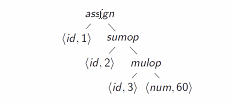
\includegraphics[width=.5\textwidth]{final-example-parsing-tree.png}
    \caption{Parsing tree ricavato dal nostro esempio}
    \label{fig:last-ex-parse-tree}
\end{figure}
Relativamente all'analisi sintattica abbiamo studiato ed utilizzato le due famiglie principali di metodi di parsing (basate su derivazioni leftmost in un caso e rightmost nell'altro). 
È da sottolineare però, che esistono parser adatti all'analisi di una qualsiasi grammatica libera, tuttavia questi hanno complessità minima \(n^3\) (con \(n\) lungehezza dell'input) e questo li esclude dalla nostra wishlist.
Non dimentichiamoci però che, concentrandoci principalmente sulle grammatiche regolari, i parser che abbiamo esaminato in questo corso riescono a ricavare un albero di derivazione con complessità \emph{LINEAREH}.

Le, ormai ben note, due tipologie principali di parsing, sono:
\begin{itemize}
    \item parsing top-down;
    \item parsing bottom-up.
\end{itemize} 

\subsection{Parsing top-down\\ \small{Quello bello}}
Quando ci troviamo al cospetto di grammatiche \(LL(1)\), riusciamo a ricavare il parse tree senza bisogno di backtrack utilizzando il parsing top-down.
La strategia di analisi del parsing top-down prevede di partire dalla derivazione dello start symbol e poi, utilizzando la derivazione di tipo leftmost, costruire il parse tree.
Se la grammatica è \(LL(1)\) va tutto liscio ed otteniamo l'albero di parsing in men che non si dica, se non lo è dobbiamo ricorrere al backtrack, ma noi non vogliamo che questo succeda, Larry (se nemmeno voi, come il revisore, avete capito... sorridete e annuite: non si contraddice mai un pazzo).

Abbiamo quindi visto delle caratteristiche che vogliamo evitare per assicurarci di lavorare sempre con grammatiche \(LL(1)\):
\begin{itemize}
    \item Le grammatiche \emph{ricorsive sinistre} \textbf{non} sono \(LL(1)\), abbiamo visto però come si può, in alcuni casi, trasformarle per renderle tali;
    \item Le grammatiche \emph{fattorizzabili a sinistra} \textbf{non} sono \(LL(1)\), ma come per il punto precedente aabbiamo visto come è possibile provare ad eliminare questo problema;
    \item Le grammatiche \emph{ambigue} \textbf{non} sono \(LL(1)\), perché esiste almeno una stringa nel linguaggio che può essere derivata in 2 modi diversi (entrambi leftmost).
\end{itemize}

\subsection{Parsing bottom-up\\ \small{Quello tosto}}
L'altra grossa famigliola di grammatiche che abbiamo visto contiene quelle grammatiche che possono essere analizzate tramite il parsing bottom-up, di questa famiglia siamo andati ad indagare queste tipologie di grammatiche:
\begin{itemize}
    \item \(SLR\)
    \item \(LR(1)\)
    \item \(LALR\)
\end{itemize}
Il goal dell'analisi bottom-up è sempre lo stesso, ma il modo in cui si va a ricostruire l'albero di derivazione è opposto al parsing top-down: si parte a ricostruire l'albero delle derivazioni dalle foglie e si continua fino alla radice.
\\\\
Indifferentemente dal tipo di grammatica che stiamo analizzando, il modo per ricavare il parse tree prevede sempre l'utilizzo dell'\emph{algoritmo shift-reduce}.
L'algoritmo di shift-reduce è anche'esso indipendente dal tipo di grammatica che si va ad utilizzare, tuttavia necessita della parsing table per quella particolare tipologia di grammatica.

Mentre eseguiamo l'algoritmo andiamo ad analizzare la lista di token in input: controllando token per token ed usando la parsing table come mappa, ci spostiamo nel buffer di lettura (mosse di shift) e, quando si incontra una stringa che può essere derivata da una certa produzione della grammatica, si va ad effettuare una mossa di reduce.

Se non vi sono entry multiple defined possiamo terminare l'agloritmo con successo ed ottenere alla fine il parsing tree che tanto desideriamo.

Le 3 grammatiche viste per il parsing bottom-up, si differenziano per la precisione con cui una determinata produzione viene inserita in una casella della tabella di parsing (oon lo scopo di eseguire una mossa si reduce).

La differenza tra un tipo di grammatica e l'altro è la seguente: 
\begin{itemize}
	\item utilizzando grammatiche e parsing \(SLR\) otteniamo un automa semplice e di veloce computazione, ma povero di informazioni (rischiamo di avere dei conflitti)
	\item d'altro canto, il parsing \(LR(1)\) ci fornisce degli automi molto più precisi, con dei lookahead set che ci danno molte più informazioni su quando applicare le riduzioni, ma che ci potrebbero portare ad una sovrabbondanza che porterà via molto tempo alla loro computazione (e anche spazio)
	\item tra \(SLR\) e \(LR(1)\) troviamo grammatiche \(LALR\), che ci offrono una tabella di parsing delle dimensioni di una tabella \(SLR\), ma hanno una complessità di calcolo leggermente superiore alle grammatiche \(SLR\) permettendoci di avere gli stessi lookahead set (quindi la stessa precisione) del parsing \(LR(1)\).
\end{itemize}

In realtà le possibilità non terminano qui, infatti si potrebbero ottenere delle grammatiche molto più semplici da parsare aumentantdo il numero di informazioni che si usano prima delle riduzioni, sostanzialmente incrementando il lookahead set: tali grammatiche potrebbero ad esempio essere \(LL(2)\) ed \(LR(2)\), ma la complessità per l'analisi della lista di token aumenterebbe parecchio in tal caso. La scelta privilegiata è quindi sforzarsi di trovare una grammatica \(LL(1)\) o \(LR(1)\) prima, per avere poi performance migliori.

\subsection{Quando finisce il parsing}
Se l'analisi sintattica dimostra che la stringa non è riconosciuta dal linguaggio, vi è la possibilità, nei compilatori moderni, di prevedere dei meccanismi di riconoscimento degli errori: spesso sono i compilatori stessi che suggeriscono all'utente dove si potrerebbero trovare gli errori sintattici all'interno del codice.

In caso l'analisi sia andata a buon fine, si ottiene un parse tree che indica quali riduzioni sono state effettuate ed in quale ordine.

\section{Analisi semantica}
Questa è la fase in cui si va a valorizzare la sequenza di token che si ricava dall'analisi lessicale; nel nostro caso quello che otterremo dall'analisi semantica ha questa forma:
\begin{figure}[H]
    \centering
    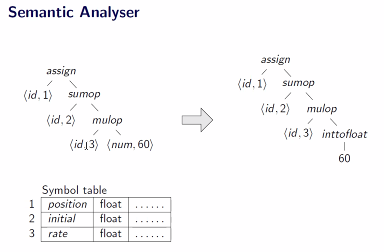
\includegraphics[width=.7\textwidth]{final-example-semantic-output.png}
    \caption{Output dell'analisi semantica}
    \label{fig:last-ex-semantic-output}
\end{figure}
Si noti che il \(<num, 60>\) è stato trasformato in \texttt{inttofloat} con nodo figlio \(60\): questo è avvenuto perchè l'analisi semantica è quella che si occupa di attribuire un valore (e di conseguenza anche un tipo) ai token. Proprio per questo motivo, gli effetti dell'analisi semantica non si vedranno solo nell'albero, come mostrato in Fig.\ref{fig:last-ex-semantic-output}, ma anche nella tabella dei simboli che riportiamo qui:
\begin{table}[H]
	\centering
	\subimport{assets/tables/}{symbol-table-updated.tex}
    \caption{Symbol table aggiornata dall'analisi semantica}
    \label{tab:last-ex-symbol-table-updated}
\end{table}
Si può immaginare, facendo qualche semplificazione, che da qualche parte nel codice, precedente a quella che stiamo analizzando noi nel nostro esempio (che ricordiamo è scritta in Eq.\ref{eq:last-ex}), avessimo dichiarato le variabili: quando l'analisi semantica raggiunge tale dichiarazione effettua una tipizzazione degli identificatori, che è appunto riportata nella tabella appena mostrata.

In seguito alla tipizzazione degli identificatori, l'analizzatore semantico, vedendo che \(rate\) è di tipo float, capisce che la moltiplicazione \(rate * 60\) deve essere di tipo float e converte \(60\) con l'operazione \texttt{inttofloat}.

Aggiungiamo inoltre che la tipizzazione che viene effettuata in questa fase, serve anche a calcolare gli offset necessari per la memorizzazione delle variabili che verrà effettuata al momento dell'esecuzione del programma: proprio grazie a questa manovra il compilatore riesce a descrivere che al tal programma servirà una quantità di memoria \(x\) per memorizzare una variabile di tipo \(y\).

A questo punto si passa alla generazione del codice intermedio.

\section{Generazione del codice intermedio}
Un modo molto semplice per ottenere la generazione del codice intermedio consiste nell'attraversare l'albero sintattico, associando un temporaneo per ogni nodo intermedio.
Si può osservare l'utilizzo di questa strategia applicata al nostro esempio: riportiamo dunque di seguito il codice intermedio generato partendo dal risultato dall'analisi semantica (Fig.\ref{fig:last-ex-semantic-output}).
\begin{align*}
    t1 &= inttofloat(60) \\
    t2 &= id3 * t1 \\
    t3 &= id2 + t2 \\
    id1 &= t3 \\
\end{align*}
Una cosa a cui prestare attenzione è il fatto che gli identificatori \texttt{id1}, \texttt{id2} e \texttt{id3} sono riferimenti alle istanze locali degli identificatori: ciò vuol dire che si entra già nel territorio per cui si necessita di un meccanismo di \emph{scope}, ma di questo parleremo in seguito.

A questo punto si passa all'ottimizzazione del codice intermedio, fase che ha le sue basi teoriche in solidissime e sofisticate prove matematiche.

\section{Ottimizzazione del codice intermedio}
Nell'esempio che stiamo trattando si riesce ad ottimizzare il codice riducendo subito il \(60\) in float ed eliminando operazioni temporanee non strettamente necessarie. Vediamo subito come risulterebbe un'ottimizzazione fatta secondo queste prerogative:
\begin{align*}
    t1 &= id3 * 60.0 \\
    id1 &= id2 + t2 \\
\end{align*}
Questa fase di ottimizzazione sfrutta algoritmi su grafo facendo un'analisi di catene di \emph{definition use}: tenendo conto del momento della dichiarazione e dell'utilizzo di una certa variabile, è possibile ad esempio decidere di eliminare o spostare tale dichiarazione.

Un esempio piuttosto comune è la \emph{subexpression elimination}, che prevede di sintetizzare tutte le espressioni che vengono ripetute nel codice: se nel nostro programma andiamo a calcolare più volte l'espressione \(\pi * e\), la subexpression elimination va a salvare in una variabile temporanea il risultato, così da evitare di calcolarlo più e più volte sprecando risorse.

Nota che tutte queste ottimizzazioni avvengono a tempo di compiliazione, nella fase statica, e sono di tipo conservativo. Questo significa che alcune occorrenze della stessa espressione possono essere eseguite in entrambi i rami di un else, quello che si fa in questo caso è assumere in modo conservativo che possano essere percorsi tutti i rami di tutte le condizioni.

In sostanza le ottimizzazioni che vengono effettuate in questa fase ottimizzano in modo cieco, senza guardare i possibili flussi di esecuzione della logica del programma.

Nota anche che nelle fasi successive tutte le variabili dovranno essere inserite nei vari registri: qui avverranno ulteriori ottimizzazioni, ad esempio legate ad un migliore utilizzo dei registri, che andranno ad utilizzare algoritmi di graph coloring e altre stregonerie simili.

A valle dell'ottimizzatore del codice intermedio abbiamo la generazione del codice target.

\section{Generazione del codice target}
A questo punto possiamo finalmente tradurre il codice intermedio in codice target. Riportimo in seguito quello che otteniamo a seguito di questa fase dal nostro esempio.
\begin{figure}[H]
    \centering
    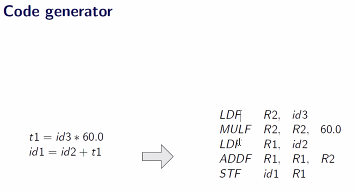
\includegraphics[width=.6\textwidth]{final-example-target-code.png}
    \caption{Generazione codice target da codice intermedio ottimizzato}
    \label{fig:final-example-target-code}
\end{figure}
Spiegamo qualche dettaglio: il suffisso \texttt{F} sta per \texttt{float} per sottolineare che tutte le operazioni coinvolgono dei float e, per questo motivo, è necessario ad esempio trattarli in maniera distinta dagli int. Possiamo osservare che nella prima riga viene caricato il contenuto di \texttt{id3} come float nel registro \texttt{R2}, poi avviene una moltiplicazione tra float che coinvolge \texttt{R2} e \(60\); segue un'operazione di \texttt{load} di un altro float e così via.

L'ultima nota che aggiungiamo riguardo a questa fase è che, come già accennato precedentemente, anche qui intevengono meccanismi di ottimizzazione, in questo caso strettamente legati al codice macchina (e quindi alla macchina target).

\section{Approfondimento sulla tabella dei simboli}
Le tabelle dei simboli vengono utilizzate fin dell'analisi lessicale e vengono mantenute per l'intera durata del processo; si capisce bene che sono le strutture principali in un compilatore, seconde solo agli alberi di parsing.

Ma come sono implementate effettivamente? 

Ci sono varie strategie in realtà, ma la più diffusa è sicuramente la struttura dati dizionario, che deve presentare queste operazioni:
\begin{itemize}
    \item insert
    \item lookup
    \item delete
\end{itemize}
I dizionari possono essere ottenuti sia con l'utilizzo di liste che con alberi di ricerca, ma l'implementazione di gran lunga più diffusa si basa sulle hash table, che offrono un costo di gestione lineare.

In questo caso si ha il canonico array bucket, da cui è possibile accedere ad una lista di elementi che contengono tutte le entry (gli elementi della tabella dei simboli) per cui la funzione di hash restituisce lo stesso risultato.

\paragraph{Funzione di hash} Com'è strutturata solitamente una funzione di hash per la tabella dei simboli di un compilatore?
Questa si occupa di trasformare ogni carattere in un intero non negativo, tipicamente sfruttando funzioni built-in, a cui applica ulteriori operazioni per poi arrivare all'hash.

Come si può definire una funzione di hash adeguata?
Conoscendo il dominio di applicazione. Ad esempio, nel nostro caso si può notare che spesso nella scrittura dei programmi, il programmatore va a dare nomi molto similli alle variabili: questo significa che utilizzare il suffiso degli identificatori non è una buona idea perchè porterebbe a diverse collisioni.

Una scelta tipicamente buona è la seguente
\begin{equation}
    (\sum_{i=1}^{n} \phi^{n-i}c_i) \; mod \; \texttt{size}
\end{equation}
Utilizzando funzioni hash di questo tipo si possono evitare con buona probabililtà le problematiche legate alla scarsa fantasia del nostro amico programmatore.

\paragraph{Scope} Ora che abbiamo discusso le metodologie di implementazione di una symbol table, andiamo ad analizzare una problematica con cui tutte devono fare i conti: lo \emph{scoping}.

Le dichiarazioni di fatto possono essere di due tipi: locali o globali.
Va quindi capito, nel caso vi siano più dichiarazioni di una variabile, a quale scope si riferiscano le sue occorrenze nel codice.
Può essere utile immaginare un AST che rappresenta un certo programma in cui lo stesso nome è utilizzato sia per una variabile globale che per una variabile locale di una subroutine.
In questo ast la variabile locale sarà in un sottoalbero dell'albero in cui è dichiarata la variabile globale; le dichiarazioni locali sono comprese in sottoalberi dell'AST.

Come si va a gestire la tabella dei simboli per rispettare lo scope delle dichiarazioni?
\noindent
Esistono due principali soluzioni per gestire queste dichiarazioni annidate:
\begin{itemize}
    \item si usa un'unica symbol table e, nella lista a cui si accede dal bucket, si va a prendere il primo elemento con lo stesso nome di quello della variabile. In questo modo si è sicuri di ottenere la variabile con scope più vicino all'occorrenza che si sta analizzando, perché la entry che è stata inserita per ultima sarà la prima della lista del bucket; adottando questa strategia però si deve anche implementare un meccanismo di rimozione delle variabili di uno scope quando si esce da quest'ultimo;
    \item creiamo una tabella dei simboli diverse per scope, in questo modo quando usciamo da uno scope ci basta cancellare il puntatore alla tabella dei simboli associata.
\end{itemize}

\section{Note finali per progetti futuri}
Il lettore deve sapere che esistono dei tool per la creazione di analizzatori sintattici, che richiedono venga fornito in input:
\begin{itemize}
    \item una grammatica;
    \item la lista di token della grammatica; 
    \item come questi token devono interagire con l'analizzatore lessicale.
\end{itemize}
Una volta che si danno questi elementi in pasto al tool, si ottiene un analizzatore sintattico bello che funzionante. Addirittura, spesso si trovano coppie di tool per la creazione di analizzatori sia lessicali che sintattici, come ad esempio la coppia di software Flex e Bison.
\\\\
Ma non è finita qui.

In alcuni casi i tool di cui sopra accettano come input anche delle funzioni di attribuzione che ci permettono di specificare le azioni semantiche per le varie produzioni (tipicamente in qualche linguaggio come il C), il che ci permette di ottenere dei parser che compiono anche la valorizzazione semantica (grazie Bison).
\\\\
Cosa significa tutto questo?

Se abbiamo un generatore di analizzatore sintattico ed un'implementazione di symbol table riusciamo a generare il nostro front-end del compilatore, poi siccome l'intermediate code può essere un qualsiasi linguaggio (spesso anche C) possiamo ottenere un compilatore in pochi semplici passi.

Alla fine quello che serve sono un generatore di analizzatori sintattici, una symbol table e due pezzi di pane del giorno prima.

\end{document}
